\documentclass[a4paper]{article}

% Packages
\usepackage{graphicx}
\usepackage[margin=1in]{geometry}
\usepackage[utf8]{inputenc}
\usepackage[T1]{fontenc}
\usepackage[backend=bibtex]{biblatex}
\usepackage{comment}
\usepackage{hyperref}
\usepackage{amsmath}

\usepackage{CJKutf8}


\addbibresource{references.bib}

\title{Evaluation of Pre-Trained Models for Many-to-English Translation}
\author{Stefan Liemawan Adji}
\date{\today}

\begin{document}

\maketitle

\section{Introduction}

According to Ethnologue \cite{ethnologue-2024}, 7,164 languages currently exist and in use today, with 40\% of them considered endangered. As of July 2024, 243 languages are supported by Google Translate (according to Wikipedia \cite{wikipedia-google-translate}). In modern times, the need for translation services has surged due to the growing exchange of information across different regions that speak various languages \cite{okpor-2014-machine-ta}.

Machine translation (MT) is the task of automatically translating from one language to another. This can be done through text or audio. It can be traced back to 1949 \cite{weaver-1999}, with the first public demonstration of an MT system on January 7, 1954, in collaboration with IBM, where 49 Russian sentences were translated into English using a limited vocabulary of 250 words and 6 grammar rules \cite{hutchins-2006-first-mt}. However, over the next several decades, growth were limited for machine translation, with 1956-1966 considered the decade of high expectation and disillusion, and 1967-1976 dubbed 'the quiet decade' \cite{hutchins-2001-mt-50-years}. Then in 1989, the dominance of the rule-based approach has been challenged by the rise of new methods and strategies, collectively referred to as ‘corpus-based’ methods (data-driven) \cite{hutchins-1994-research-methods-mt,hutchins-1998-development-mt}. Subsequently, statistics-based approaches for MT re-emerged, bolstered by the recent success of probabilistic techniques in speech recognition. Statistical machine translation \cite{lopez-2008-smt} dominated the domain between late 1990s through the early 2010s, before largely being surpassed by neural machine translation (NMT) \cite{cho-2014-properties,sutskever-2014-seq2seq}.

Since the introduction of Transformers in 2017 \cite{vaswani-2017-attention}, Natural Language Processing (NLP) and machine translation in particular reached a giant milestone. The following years saw the birth of Large Language Models (LLMs) such as BERT \cite{devlin-2019-bert}, GPT \cite{openai-2024-gpt4}, and T5 \cite{raffel-2023-t5}, which revolutionised both MT and the whole field of NLP. Then in early 2020s, several pre-trained models (PTM) that are specifically designed for machine translation emerged, namely mBART \cite{liu-2020-mbart}, mT5 \cite{xue-2021-mt5}, NLLB \cite{nllb200-2020}, M2M \cite{fan-2020-m2m100}, and PolyLM \cite{wei-2023-polylm}. Most of these models are multilingually trained, allowing for many-to-many translation: able to translate between any of the supported pair of languages. This allows the models to generalise over shared lexical and linguistic among languages, and have been shown to increase performance compared to one-to-one translation models \cite{liu-2020-mbart}.

Intento published 'The State of Machine Translation 2024' \cite{intento-2020} providing an in-depth evaluation of popular MT engines and LLMs. However, the biggest drawback in this report is that the selected LLMs are general LLMs such as GPT, LLaMa, Mistral, instead of MT-specific LLMs.

Despite these advancements, pre-trained models are often evaluated using different set of benchmarks \cite{liu-2020-mbart,nllb200-2020,fan-2020-m2m100,wei-2023-polylm}, making it difficult to gauge their relative effectiveness across various languages. Nevertheless, there does not seem to be much work on comparing or benchmarking different pre-trained models in machine translation.

Through simple experimentations, this paper aims to evaluate the performance of existing pre-trained models (PTMs) on many-to-English translation across 14 source languages. Although fine-tuning multilingual PTMs has been proven to increase model performance \cite{cooper-stickland-2021-recipes}, no pre-training or fine-tuning is performed in this study for simplicity reasons. A dataset is curated from the Tatoeba repository \cite{tatoeba}, containing 1,323 parallel sentence pairs across source and target languages. The models includes a one-to-one PTMs: OPUS-MT \cite{tiedemann-2023-democratizing,tiedemann-2020-opus-mt}, and multilingual PTMs: such as mBART-50 \cite{liu-2020-mbart}, NLLB-200 \cite{nllb200-2020}, and M2M-100 \cite{fan-2020-m2m100}. The performance of these models is evaluated using the BLEU score \cite{papieni-2002-bleu}.


% (Multilinguality has been explored in the supervised NMT literature, where it has been shown to enable information sharing among related languages.) \cite{garcia-2020-multilingual}
% (NMT systems have lower translation quality on very long sentences) \cite{koehn-2017-challenges}


\section{Literature Review}

\subsection{Pre-Trained Models for Machine Translation}

The encoder-decoder approach \cite{cho-2014-properties} remains as the foundation architecture for many sequence-to-sequence models in machine translation.

In terms of pre-trained models (PTMs) for machine translation, it can be divided into two categories: one-to-one models and many-to-many models (multilingual).

One-to-One Translation refers to a translation approach where a model is specifically trained to translate between one source language and one target language. This setup is characterised by having a dedicated model for each unique language pair. An example of this setup is OPUS-MT by Helsinki-NLP \cite{tiedemann-2023-democratizing,tiedemann-2020-opus-mt}, which provides over 1,000 pre-trained models for translation between numerous language pairs.

With the advent of large language models and pre-trained language models, multilingual machine translation has gained prominence. This approach enables many-to-many translation, where a single model can translate between multiple source and target languages \cite{aharoni-2019-massively-multilingual}. mBART \cite{liu-2020-mbart} is a sequence-to-sequence denoising auto-encoder model specifically designed for multilingual tasks. The mBART-50 variant supports many-to-many translations for over 50 languages. M2M-100 \cite{fan-2020-m2m100} is designed to perform direct translation between 100 languages without relying on English as an intermediate language. NLLB-200: NLLB-200 \cite{nllb200-2020} is built to handle translation tasks across a broad spectrum of languages, including many that are low-resource or underrepresented in existing datasets. It supports translations for 200 languages, encompassing numerous underrepresented languages. mBART, M2M-100, and NLLB-200 were all developed by Meta AI (formerly Facebook AI), showcasing the organisation's significant impact in the machine translation field through pre-trained models (PTMs). These models represent a substantial advancement in multilingual translation capabilities.

\subsection{Parallel Corpora}

Corpora are large and structured sets of texts used for linguistic research and analysis. Thus, parallel corpora are defined as sets of texts in a given source language along with their translations in another target language \cite{lefer-2020-parallel-corpora}. It can be bilingual or multilingual, and are crucial for training and evaluating machine translation. Languages without or with limited parallel corpora are referred as \textbf{low-resources language}.

Since the early 2000s, English has often been used as an intermediary language, meaning texts originally written in languages are first translated into English, and then from English into other languages, resulting in most target texts being translations of translations \cite{lefer-2020-parallel-corpora}. This is called indirect translation, and posed for many problems in translations as terms can be ambiguous with varying or similar meanings \cite{rosa-2017-indirect-translation-problems}.

Neural Machine Translation (NMT) systems require vast amounts of training data, and thus the availability of parallel corpora is crucial for building effective models \cite{koehn-2017-challenges}. The lack of extensive parallel corpora, especially for low-resource languages, leads to suboptimal performance in NMT techniques compared to their high-resource counterparts \cite{ranathunga-2023-nmt-low-res}. OPUS \cite{opus} is a comprehensive collection of open-source parallel corpora used extensively in the field of machine translation (MT). It includes corpora for 744 languages and contains over 1,210 different datasets, amassing a total of 45,945,946,108 sentence pairs. Tatoeba \cite{tatoeba} is another prominent resource in the field of MT and NLP, known for its extensive collection of translated sentences. As of July 2024, it contains 12,186,207 sentences over 423 supported languages, growing daily through volunteer contributions.

Several datasets are often used for evaluation in machine translation. The Tatoeba Challenge \cite{tiedemann-2020-tatoeba-challenge} covers 487 languages in 4,024 language pairs, including 657 test sets sourced from Tatoeba website, covering 138 languages. The TED Talks dataset \cite{ye-2018-word-embeddings-ted} contains transcripts from TED talks for more than 50 languages. IWSLT \cite{agarwal-iwstl-2023} also contains TED talks data, but paired with English translations. Finally, WMT \cite{barrault-2020-wmt} is an annual event that organises tasks for machine translation and provides a collection of datasets for benchmarking and evaluating translation systems.

While these datasets can be used to evaluate translation performance between any language pairs, they do not contain parallel corpora between different languages. Corpus between English and French for example, contains different text to the corpus between English and Spanish. Therefore, they do not support easy evaluation for many-to-English translations.

Furthermore, papers often use different sets and different versions of datasets to evaluate their model performance, incurring unstraightforward comparison.

mBart \cite{liu-2020-mbart} uses WMT19 for English-German translation and TED15 for Chinese-English translation. M2M-100 \cite{fan-2020-m2m100} uses 7 different datasets shared across languages. NLLB-200  \cite{nllb200-2020} uses FLORES dataset, designed for low-resources languages. OPUS-MT \cite{tiedemann-2023-democratizing,tiedemann-2020-opus-mt} models use datasets from Tatoeba challenges.


\subsection{Evaluation Metrics}

Other metrics for machine translation exist, but not used nearly as widely as BLEU. Crosslingual Optimized Metric for Evaluation of Translation (COMET) \cite{rei-2020-comet} is a recent metric that leverages neural-network-based models for deeper understanding and evaluation. BERTScore.

In this project, a variant of BLEU called SacreBLEU and METEOR will be used due to their simplicity.


\subsubsection{BLEU}

Bilingual Evaluation Understudy (BLEU) \cite{papieni-2002-bleu} is the most commonly used metrics for machine translation (MT). It assesses how well a candidate translation matches the reference translation using precision metrics for n-grams and incorporates a brevity penalty to prevent overly short translations from achieving high scores.

The n-gram precision, as presented in the original BLEU paper \cite{papieni-2002-bleu}, is calculated as:

\begin{equation}
    p_n = \frac{\sum_{C \in \{Candidates\}} \sum_{\text{n-gram} \in C} \text{Count}_{\text{clip}}(\text{n-gram})}{\sum_{C \in \{Candidates\}} \sum_{\text{n-gram} \in C} \text{Count}(\text{n-gram})}
\end{equation}

Where:
\begin{itemize}
    \item \( p_n \) is the precision for n-grams.
    \item \( \sum_{C \in \{Candidates\}} \) denotes the summation over all candidate translations.
    \item \( \sum_{\text{n-gram} \in C} \) denotes the summation over all n-grams in a candidate translation \( C \).
    \item \( \text{Count}_{\text{clip}}(\text{n-gram}) \) is the clipped count of the n-gram, which is the count of the n-gram in the candidate translation limited by the maximum count of that n-gram in any reference translation.
    \item \( \text{Count}(\text{n-gram}) \) is the count of the n-gram in the candidate translation.
\end{itemize}

Thus, the BLEU score is calculated as:

\begin{equation}
    \text{BLEU} = BP \cdot \exp \left( \sum_{n=1}^{N} w_n \log p_n \right)
\end{equation}

Where:
\begin{itemize}
    \item \( BP \) is the brevity penalty.
    \item \( p_n \) is the precision for n-grams.
    \item \( w_n \) is the weight for each n-gram (often uniformly distributed, so \( w_n = \frac{1}{N} \)).
\end{itemize}

The brevity penalty (BP) is calculated as:

\begin{equation}
    BP = \begin{cases}
        1                     & \text{if } c > r    \\
        e^{(1 - \frac{r}{c})} & \text{if } c \leq r
    \end{cases}
\end{equation}

Where:
\begin{itemize}
    \item \( c \) is the length of the candidate translation.
    \item \( r \) is the effective reference length.
\end{itemize}

The machine translation community's rely heavily BLEU score, however, it has several drawbacks. The metric has been reported to not correlate strongly with human judgement, showing variations in translation that could mean that a higher BLEU score does not necessarily indicate a true enhancement in translation quality \cite{callison-burch-2006-reevaluating-bleu}.

Furthermore, It is challenging to directly compare BLEU scores between paper \cite{post-2018-clarity-bleu}. Thus, the author proposed a variation called SacreBLEU \cite{post-2018-clarity-bleu}, which claimed to facilitate easy computation of BLEU scores that are shareable, comparable, and reproducible. This is done by including preprocessing steps and normalisation routines.


\subsubsection{METEOR}

Metric for Evaluation of Translation with Explicit ORdering (METEOR) \cite{lavie-2007-meteor} assesses a translation by calculating a score that reflects explicit word-to-word matches between the reference and a candidate translation \cite{agarwal-2008-meteor-mbleu-mter}. It is designed to address some limitations of the BLEU score, allowing matches between simple morphological variants and synonyms.

\begin{equation}
    \text{METEOR} = (1 - \gamma \cdot \text{frag}) \cdot \frac{P \cdot R}{\alpha \cdot P + (1 - \alpha) \cdot R}
\end{equation}

Where:
\begin{itemize}
    \item \(P\) is the precision,
    \item \(R\) is the recall,
    \item \(\text{frag}\) is the fragmentation penalty,
    \item \(\gamma\) is a parameter that controls the weight of the fragmentation penalty, commonly 0.5,
    \item \(\alpha\) is a parameter that controls the balance between precision and recall, commonly 0.9,
\end{itemize}



\section{Experiments}

\subsection{Dataset}

Tatoeba is a vast, continuously expanding database consisting sentences and their translations, built through the contributions of thousands of volunteers, offering a tool that allows users to see examples of how words are used in sentences \cite{tatoeba}. They currently have 12,132,349 sentences and 423 supported languages, with around one to two thousand new sentences added daily, on average. The English sentence dataset contains 1,905,089 sentences, the largest one in their repository, with Russian in the second place with 1,066,633 sentences. Some languages supported on the website is shown in Figure \ref{fig:tatoeba_languages} and Figure \ref{fig:tatoeba_top_bottom_languages}, sorted from the biggest corpus.

\begin{figure}[htbp]
    \centering
    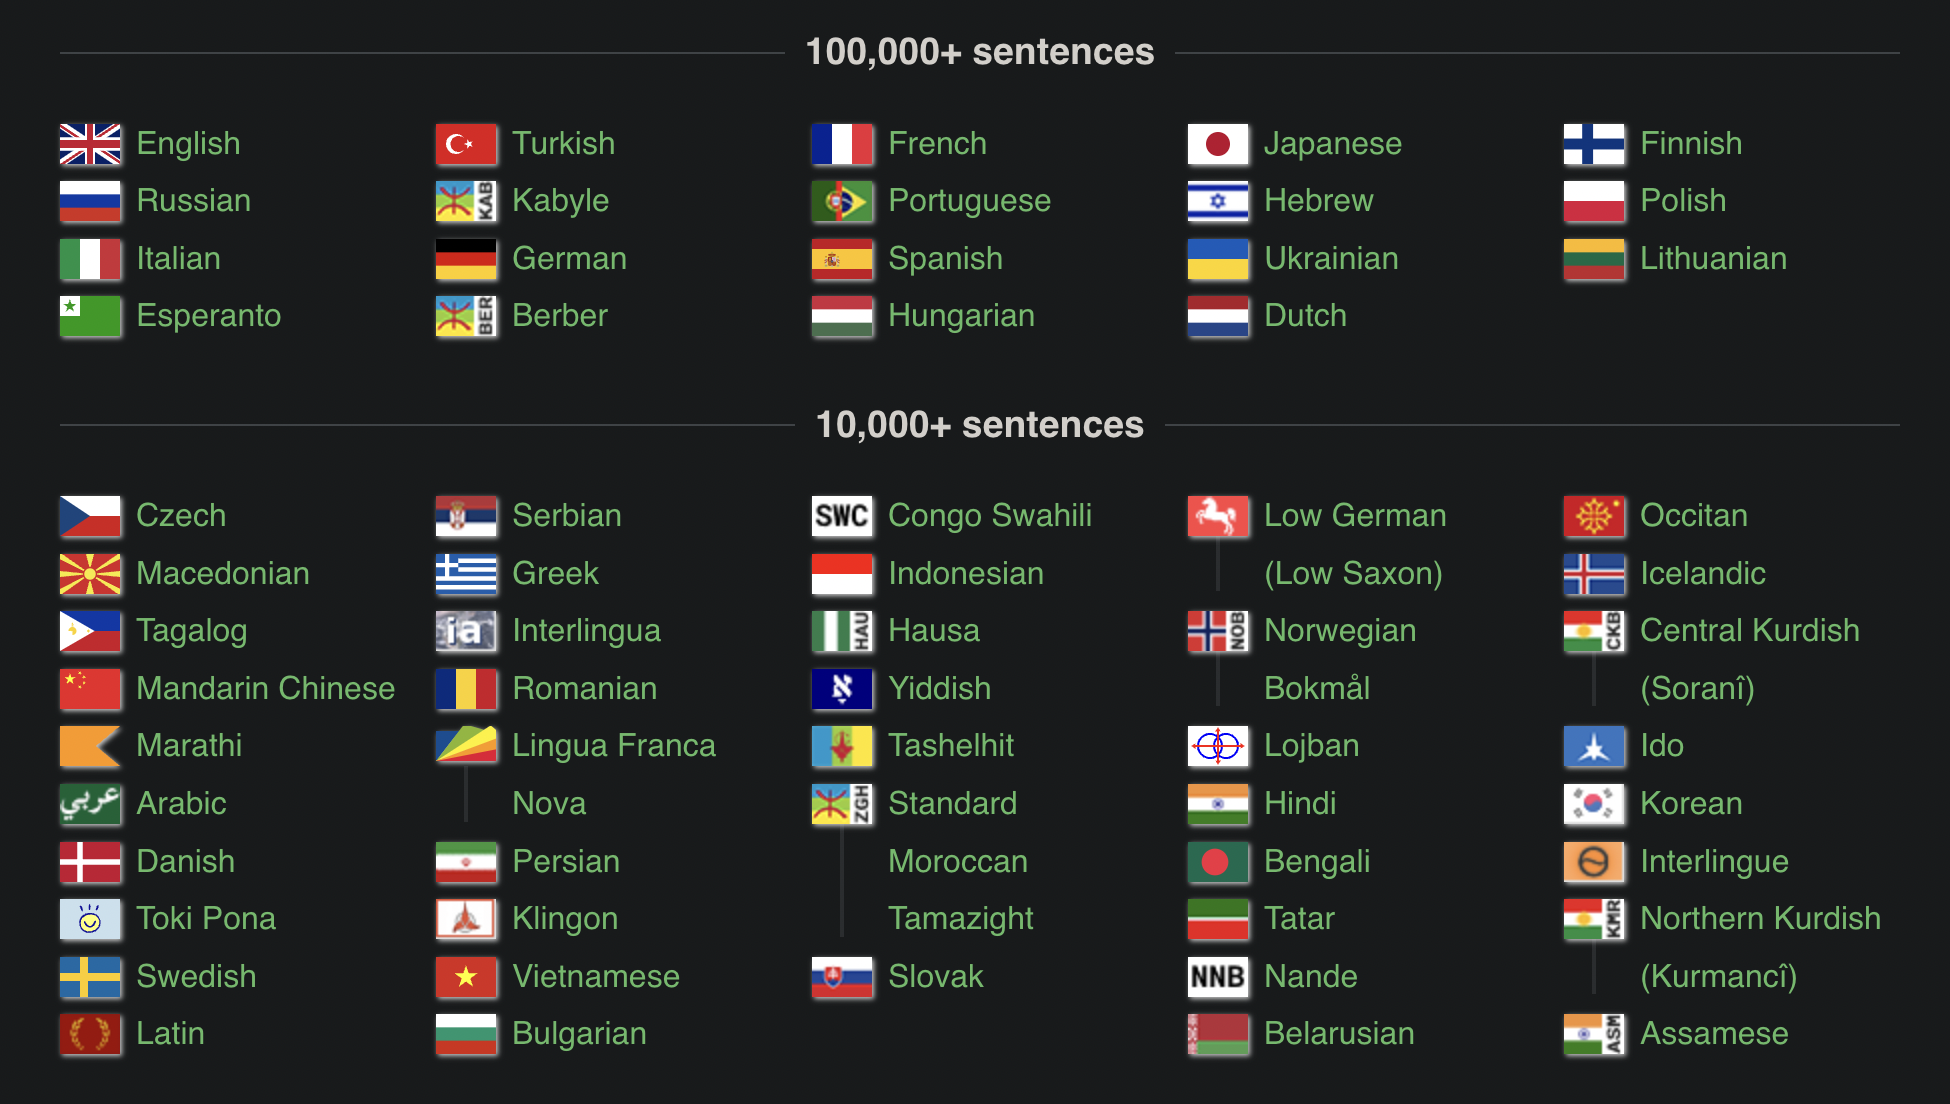
\includegraphics[width=0.9\linewidth]{images/tatoeba_languages.png}
    \caption{Tatoeba's languages repository with 10,000+ sentences and 100,000+ sentences \cite{tatoeba}}
    \label{fig:tatoeba_languages}
\end{figure}


\begin{figure}[htbp]
    \centering
    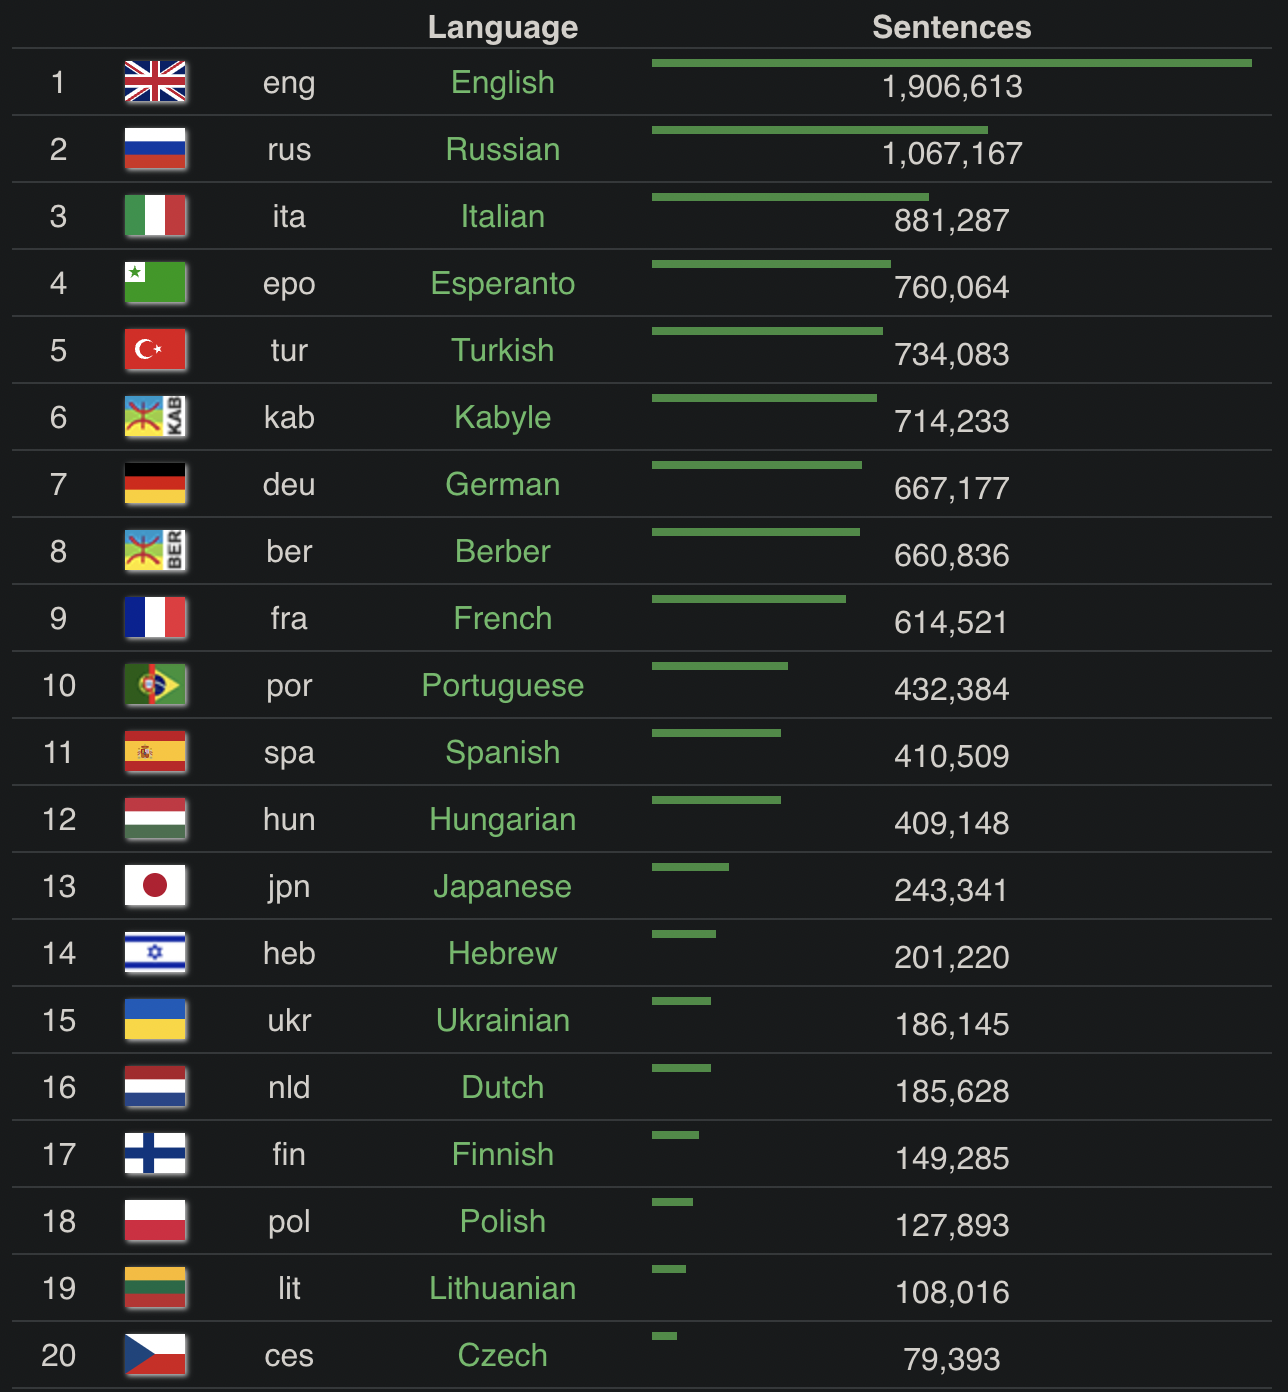
\includegraphics[width=0.5\linewidth]{images/tatoeba_top_20_lang.png}
    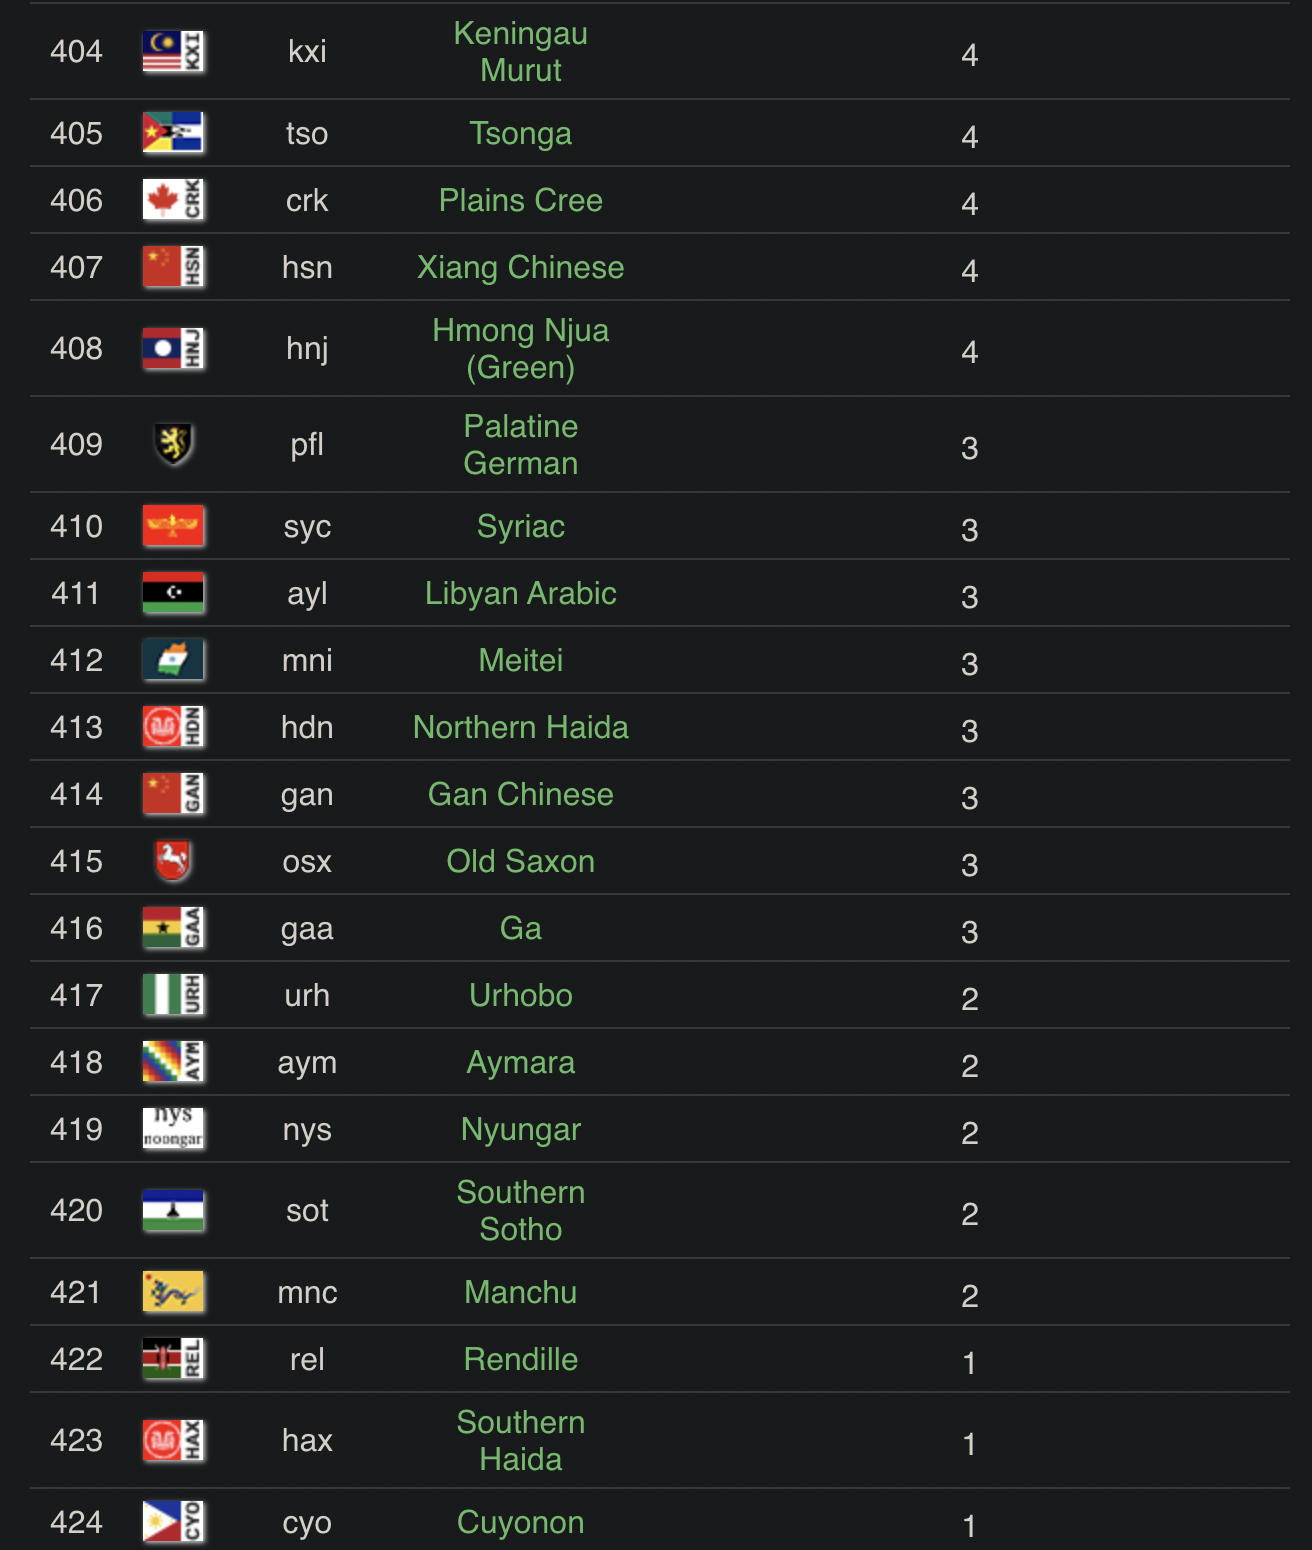
\includegraphics[width=0.46\linewidth]{images/tatoeba_bottom_20_lang.png}
    \caption{Tatoeba top 20 and bottom 20 languages based on sentences count \cite{tatoeba}}
    \label{fig:tatoeba_top_bottom_languages}
\end{figure}


\begin{table}[htbp]
    \centering
    \begin{tabular}{|l|l|r|}
        \hline
        \textbf{No.} & \textbf{Language} & \textbf{Sentence Pairs Count} \\
        \hline
        1            & Chinese           & 68,814                        \\
        2            & Dutch             & 155,856                       \\
        3            & Finnish           & 102,202                       \\
        4            & French            & 405,088                       \\
        5            & German            & 501,145                       \\
        6            & Hebrew            & 172,082                       \\
        7            & Hungarian         & 171,698                       \\
        8            & Italian           & 624,160                       \\
        9            & Japanese          & 270,116                       \\
        10           & Polish            & 77,345                        \\
        11           & Russian           & 722,837                       \\
        12           & Spanish           & 265,253                       \\
        13           & Turkish           & 710,279                       \\
        14           & Ukrainian         & 214,244                       \\
        \hline
    \end{tabular}
    \caption{List of chosen languages for evaluation}
    \label{table:eval_languages}
\end{table}

Table \ref{table:eval_languages} show the 14 languages selected for this project. Languages are chosen based on its resources' availability in Tatoeba, as well as considering supported languages in most PTMs models. To build the dataset, sentences in English are first downloaded, containing 1,898,494 sentences (it is unclear why it is less than the number stated in the Tatoeba website). Then for each language, sentence pairs between English and source languages are downloaded individually and compiled. The result is a single Dataframe containing 1,323 parallel sentences in all 14 languages, this will be treated as a test set to evaluate the models performance on each language.

Sentences typically consist of everyday phrases such as 'I have to go to sleep', 'That is intriguing', and 'Where do you live?'. They may also include single-word exclamations like 'Speak!' or 'Look!'. Additionally, multiple sentences such as 'You may write in any language you want. On Tatoeba, all languages are considered equal', and 'Guns don't kill people. People kill people' can be found inside the corpus. A few of them also include human names, 'Compare your answer with Tom's', 'Muiriel is 20 now'. All of the sentences are straightforward and literal, without the use of linguistic devices such as metaphors or sarcasm. Therefore, machine translation process should be straightforward on this level.

\begin{CJK}{UTF8}{gbsn}
    \begin{table}[htbp]
        \centering
        \begin{tabular}{|l|l|l|}
            \hline
            \textbf{Language} & \textbf{Sentence 1}                   & \textbf{Sentence 2}                   \\
            \hline
            English           & I have to go to sleep.                & So what?                              \\
            Chinese           & 我该去睡觉了。                               & 那又怎樣?                                 \\
            Dutch             & Ik moet gaan slapen.                  & Dus?                                  \\
            Finnish           & Minun täytyy mennä nukkumaan.         & Mitä sitten?                          \\
            French            & Je dois aller dormir.                 & Et alors ?                            \\
            German            & Ich muss jetzt schlafen.              & Na und?                               \\
            Hebrew            & <hidden-due-to-latex-incompatibility> & <hidden-due-to-latex-incompatibility> \\
            Hungarian         & Aludni kell mennem.                   & És akkor mi van?                      \\
            Italian           & Devo andare a dormire.                & E allora?                             \\
            Japanese          & 私は眠らなければなりませ                          & だから何?                                 \\
            Polish            & Muszę iść spać.                       & No i co?                              \\
            Russian           & Мне пора идти                         & Так что?                              \\
            Spanish           & Tengo que irme a dormir.              & ¿Entonces qué?                        \\
            Turkish           & Yatmaya gitmek zorundayım.            & Öyleyse ne yapmalı?                   \\
            Ukrainian         & Маю піти спати.                       & Ну то що?                             \\
            \hline
        \end{tabular}
        \caption{A snippet of the dataset}
        \label{table:parallel_sentence}
    \end{table}
\end{CJK}

Figure \ref{table:parallel_sentence} shows a few examples of parallel sentences in the final dataset.

\begin{figure}[htbp]
    \centering
    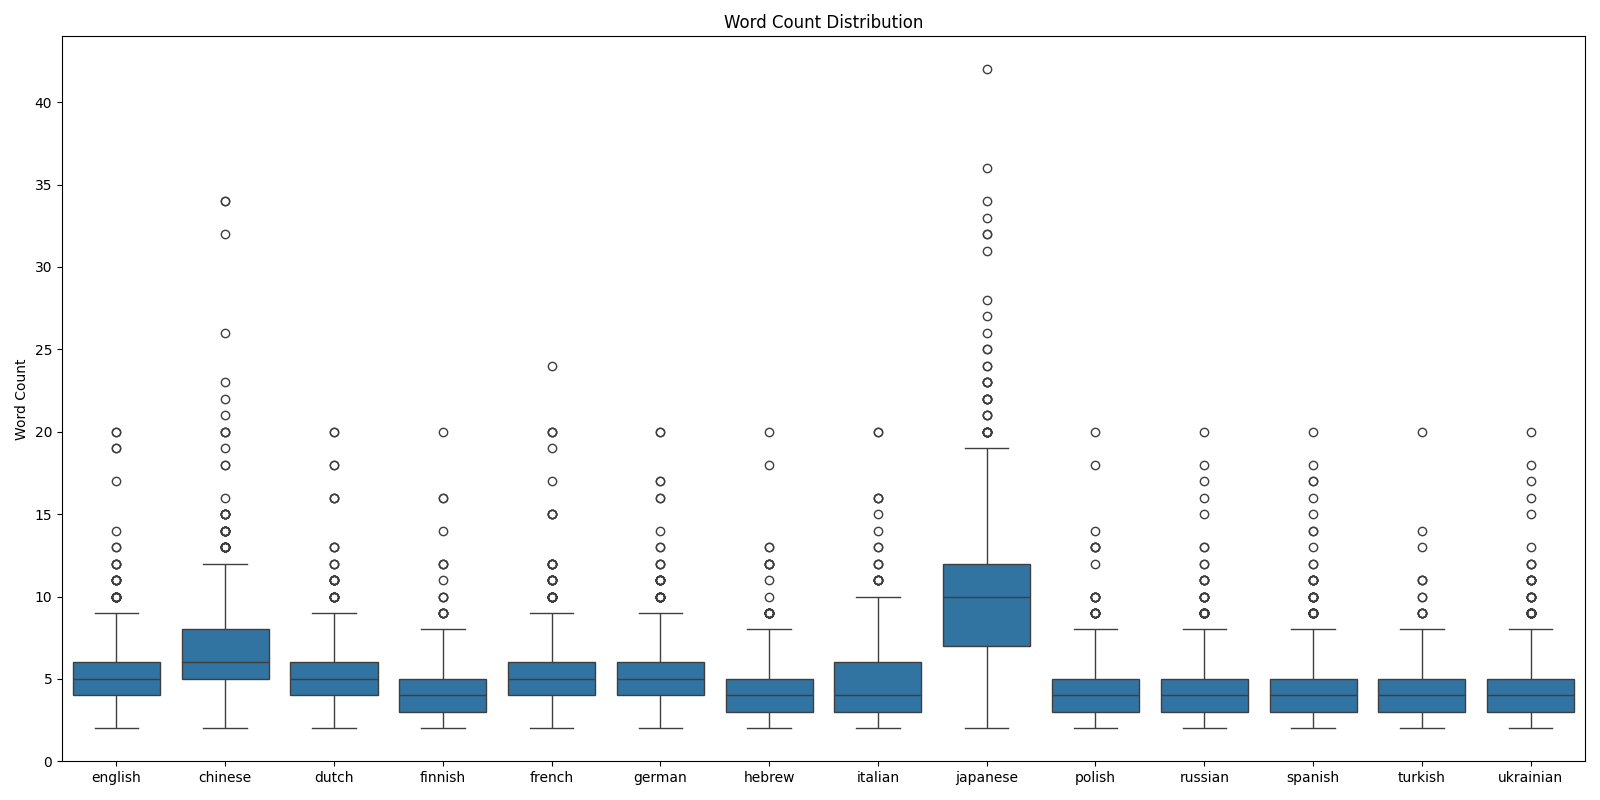
\includegraphics[width=1\linewidth]{figures/word_count_box.png}
    \caption{Dataset word count distribution, consisting of mostly short sentences.}
    \label{fig:word_count_box}
\end{figure}

Figure \ref{fig:word_count_box} shows a box plot of sentences word count. It can be seen that the majority of sentences are short.

Chinese and Japanese are counted per letter.

While most languages cluster around 4-6 words per sentence, there are notable exceptions like Japanese, which exhibits much less variability. This analysis can be useful for understanding language-specific characteristics in sentence structure, which could inform tasks like translation, text processing, or linguistic studies.

\section{Evaluation}


\begin{table}[htbp]
    \centering
    \begin{minipage}{0.49\linewidth}
        \footnotesize
        \begin{tabular}{|l|r|r|r|}
            \hline
            \textbf{Language} & \textbf{BLEU} & \textbf{SacreBLEU} & \textbf{METEOR} \\
            \hline
            Chinese           & 0.0975        & 43.3490            & 0.6848          \\
            Dutch             & 0.0976        & 52.6920            & 0.7448          \\
            Finnish           & 0.0975        & 49.9149            & 0.7145          \\
            French            & 0.0969        & 51.4090            & 0.7288          \\
            German            & 0.0969        & 52.7877            & 0.7423          \\
            Hebrew            & 0.0981        & 50.3287            & 0.7198          \\
            Italian           & 0.0975        & 53.1644            & 0.7341          \\
            Japanese          & 0.0959        & 41.6610            & 0.6511          \\
            Polish            & 0.0984        & 52.5151            & 0.7301          \\
            Russian           & 0.0976        & 48.2725            & 0.7027          \\
            Spanish           & 0.0977        & 52.9323            & 0.7371          \\
            Turkish           & 0.0978        & 51.3009            & 0.7262          \\
            Ukrainian         & 0.0978        & 46.5555            & 0.6890          \\
            \hline
        \end{tabular}
        \caption{M2M-100}
    \end{minipage}
    \begin{minipage}{0.49\linewidth}
        \footnotesize
        \begin{tabular}{|l|r|r|r|}
            \hline
            \textbf{Language} & \textbf{BLEU} & \textbf{SacreBLEU} & \textbf{METEOR} \\
            \hline
            Chinese           & 0.0962        & 54.7322            & 0.7600          \\
            Dutch             & 0.0970        & 63.6482            & 0.8007          \\
            Finnish           & 0.0963        & 47.2194            & 0.7067          \\
            French            & 0.0968        & 57.2482            & 0.7598          \\
            German            & 0.0967        & 63.1666            & 0.8022          \\
            Hebrew            & 0.0972        & 58.0846            & 0.7590          \\
            Italian           & 0.0972        & 65.9415            & 0.8068          \\
            Japanese          & 0.0943        & 43.9547            & 0.7151          \\
            Polish            & 0.0978        & 62.7550            & 0.7923          \\
            Russian           & 0.0974        & 58.8820            & 0.7686          \\
            Spanish           & 0.0883        & 35.1593            & 0.7306          \\
            Turkish           & 0.0975        & 50.9377            & 0.6982          \\
            Ukrainian         & 0.0964        & 55.8637            & 0.7496          \\
            \hline
        \end{tabular}
        \caption{mBART50}
    \end{minipage}
\end{table}


\begin{table}[htbp]
    \centering
    \begin{minipage}{0.49\linewidth}
        \footnotesize
        \begin{tabular}{|l|r|r|r|}
            \hline
            \textbf{Language} & \textbf{BLEU} & \textbf{SacreBLEU} & \textbf{METEOR} \\
            \hline
            Chinese           & 0.0949        & 50.4454            & 0.7180          \\
            Dutch             & 0.0915        & 20.8988            & 0.2899          \\
            Finnish           & 0.0921        & 32.3926            & 0.4006          \\
            French            & 0.0950        & 32.1389            & 0.4338          \\
            German            & 0.0903        & 7.1436             & 0.1528          \\
            Hebrew            & 0.0897        & 2.3455             & 0.1412          \\
            Italian           & 0.0926        & 24.2702            & 0.3059          \\
            Japanese          & 0.0842        & 1.9569             & 0.0919          \\
            Polish            & 0.0937        & 38.4395            & 0.4739          \\
            Russian           & 0.0918        & 20.6734            & 0.2977          \\
            Spanish           & 0.0929        & 26.3313            & 0.3578          \\
            Turkish           & 0.0945        & 45.2721            & 0.6187          \\
            Ukrainian         & 0.0914        & 9.0340             & 0.1613          \\
            \hline
        \end{tabular}
        \caption{NLLB-200}
    \end{minipage}
    \begin{minipage}{0.49\linewidth}
        \footnotesize
        \begin{tabular}{|l|r|r|r|}
            \hline
            \textbf{Language} & \textbf{BLEU} & \textbf{SacreBLEU} & \textbf{METEOR} \\
            \hline
            Chinese           & 0.0971        & 59.5098            & 0.7953          \\
            Dutch             & 0.0974        & 69.8803            & 0.8471          \\
            Finnish           & 0.0965        & 66.6267            & 0.8296          \\
            French            & 0.0967        & 69.8185            & 0.8357          \\
            German            & 0.0969        & 69.7422            & 0.8419          \\
            Hebrew            & 0.0977        & 66.5149            & 0.8229          \\
            Italian           & 0.0979        & 74.1298            & 0.8584          \\
            Japanese          & 0.0960        & 63.1435            & 0.7893          \\
            Polish            & 0.0952        & 61.9026            & 0.8425          \\
            Russian           & 0.0974        & 66.7046            & 0.8179          \\
            Spanish           & 0.0979        & 71.4174            & 0.8463          \\
            Turkish           & 0.0980        & 72.6551            & 0.8460          \\
            Ukrainian         & 0.0978        & 75.4447            & 0.8667          \\
            \hline
        \end{tabular}
        \caption{OPUS-MT}
    \end{minipage}
\end{table}


\begin{figure}[htbp]
    \centering
    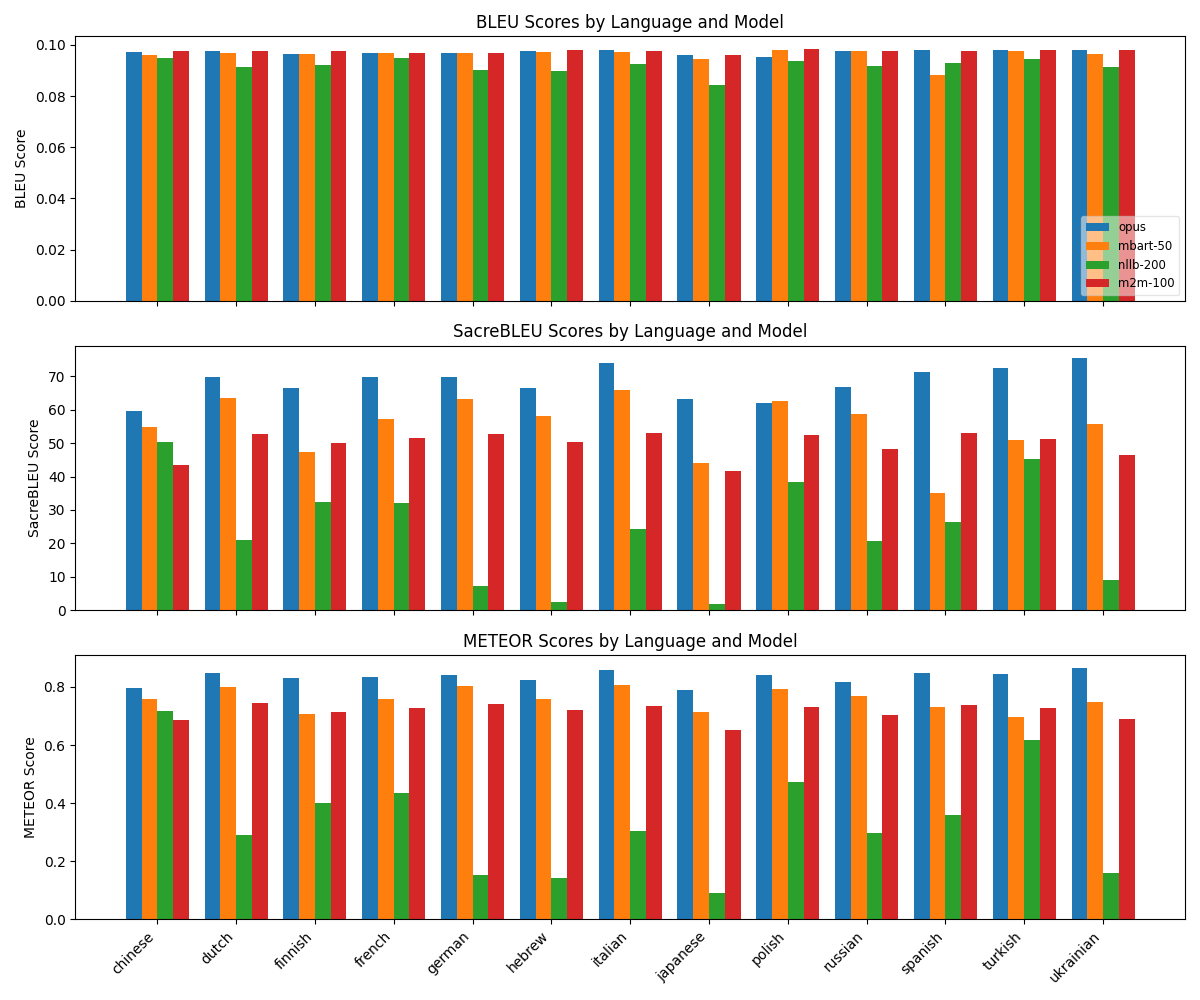
\includegraphics[width=1\linewidth]{figures/metrics_bar.png}
    \caption{BLEU, SacreBLEU, and METEOR scores of each model on each language.}
    \label{fig:result_visual}
\end{figure}

Figure \ref{fig:result_visual} shows the visualisation of all scores.

\section{Conclusion}

% READ THIS \cite{intento-2020} (exactly what this paper should do, maybe compare results and find insights)

\printbibliography
\end{document}
